\documentclass[a4paper, 12pt, openany, oneside]{book}
% Header file
% author: marcobecerrap
% date: January-2015

\usepackage{cite} % Citation Package
\usepackage{natbib} % Citation style
\usepackage{graphicx} % Graphics Package
\usepackage{amssymb, amsmath, amsbsy} % Equations
\usepackage{caption}
\usepackage{subcaption}
%\usepackage[utf8]{inputenc} % Special characters (e.g. spanish accents).
 % Included packages located in a separate file
\pagestyle{plain} %Page numbers on the bottom

\begin{document}

% Front page
\pagestyle{emty} %No numbers
\begin{titlepage}
\begin{center}

	{UoB, CS}\\
	{Report 3}\\
	{Title: SM of HE with a MR}\\
	{Student: MABP}\\
	{Supervisor: NH}\\
	{Thesis Group: JW & PH}

\end{center}
\end{titlepage}

\cleardoublepage

% Table of Contents
\newpage
\pagenumbering{roman}
\tableofcontents

% Main Chapters
\newpage
\pagestyle{plain}
\pagenumbering{arabic}
% Abstract
\chapter{Introduction}

% INTRO 
% > Robots in everyday environments are important.
% > This environment is hard.
% > Robots needs cognitive skills: understand the environment.
\section{Introduction}
One of the main goals in AI is having robots working autonomously in everyday environments. 
In such situation, robots are expected to perceive, understand and interact with its environment. 
However, these kind of environments are dynamic, non-structured and non-deterministic, which makes difficult for a robot to fulfil the assigned tasks. 
To be able to sort these obstacles, robots need to be provided with cognitive skills.

Human cognition refers to all mental activities associated with thinking, knowing, remembering and communicating, and how the information is processed \citep{King2014Psychology,myers2013psychology}. 
In robotics, the concept is associated with systems that emulate these mental processes or those that \textit{sense}, \textit{plan} and \textit{act}.
More precisely, cognition can refer to those systems that can perceive, understand \ldots and interact with their environment, and evolve in order to achieve human-like performance in activities requiring context (situation and task) specific knowledge \citep{christensen2010cognitive}.

% GENERALITIES ABOUT HUMAN ACTIVITIES
% > Activities are important part of the scenes and they are necessary to be able to understand the scene
% > Activities are entities with a spatio-temporal & symbolic (semantic, hierarchical) characteristics
Everyday environments have many valuable features that a robot needs to understand, in order to succeed while performing a task, among them are human activities.
Human activities are a meaningful manifestation of human behaviour along time and space. %TODO Expand the definition of activity.
They provide rich information about the human performing it, but also, about his/her relation with other relevant components of the environment as humans, objects and locations.


%\section{Research Problem}
\subsection{Human activity analysis with a mobile robot}
% ACTIVITY RECOGNITION
% > AR as a field
% > Robot case, advantages and disadvantages of using a robot
Activity recognition is the research field that studies the automatic detection and analysis of human activities by processing the data acquired from sensors \citep{Aggarwal14_HumActRec3DRev}. 
It is not restricted only to sensory data and this can also be complemented with other sources of information, i.e. domain knowledge.
In the AI context, activity recognition is closely related with the areas of perception, knowledge representation and reasoning. 
The problem of activity recognition has been treated from different perspectives, however, computer vision has been the most popular.

% Robots in AR (general)
In principle, robots with appropriate sensing and processing capabilities can perform activity recognition. 
Moreover, they have some advantages over the use of fixed cameras or wearable devices as they are able to interact with the environment. 
Robots are active observers, i.e. they can change their point of view on scene and be selective in the areas of the environment that are more interesting. 
On the other hand, they have some disadvantages as well. 
They don't have omnipresence, so they are not able to sense the full environment and will loose information.
Also, their sensors have constraints, the data may be noisy or blurry due to movement, erratic hardware, changing environmental conditions, etc. 
Finally, robots are expected to work in real-time, so online activity recognition is desirable but yet difficult to achieve.

% BRIDGE TO ASP
Activities involve knowledge.
They associate concepts and relations between a subject and the environment.
In general, an activity recognition system should be able to handle, not only sensory data but also symbolic representations, and be able link top level symbolic concepts to low level sensory data; this is known as the \textit{anchoring problem} \citep{Coradeschi03_AnchoringProblem}.
With this in mind, knowledge processing and reasoning is a necessity for such systems.


\subsection{Answer Set Programming for Knowledge Representation and Reasoning}

There have been proposed many ideas to handle the problems of knowledge representation and reasoning (e.g. logic programming, ontologies, bayesian networks, fuzzy logic, etc.), among them is Answer Set Programming (ASP).
ASP is form of declarative programming oriented towards difficult, primary NP-hard, search problems.
It establish a new paradigm of logic programming that allows concepts as negation as a failure, default knowledge and non-monotonic reasoning.

ASP main concepts were proposed since the late 1980s \citep{Gelf88a} and it has been used with success in many applications.
Traditionally, ASP solvers were designed as one-shot problem solvers, so they lacked of reactive capabilities and, for example, whenever new data arrived, the system needed to be restarted.
This has been one of the main reasons why ASP has not been fully exploited in the field of robotics, however, in recent years an important effort has been directed towards this direction by some groups \citep{AndresOSSR13_rosoclingo,Erdem2013_IntLowRTaskP}.


\section{Research Problem}

This project is based in the consideration of ASP as a solid option for robots in problems that require symbolic representations.
The focus of this project is to study \textbf{ASP-based activity recognition with a mobile robot}. The interest lies  in the spatio-temporal relation between human activities and the environment and how a robot can acquire, handle and use this knowledge.

ASP allows the manipulation of incomplete information and handling multiple sources of knowledge.
The integration between observations and external knowledge appear to be a more robust approach than a single sensory based approach.
Hardware adds uncertainty via noise, is constrained by its specification and the outcome data is usually difficult to process.
This uncertainty cannot be eradicated in robots, but the treatment of some problems as activity recognition can be boosted by emphasizing a more cognitive approach. 
%(via) the it can be  by emphasizing cognitive mechanisms By putting emphasis in the cognitive essence of the problem of activity recognition, the uncertainty in the cognitionemphasizing aputting emphasis in athe upper layer of knowledge representation and reasoning in solving problems that require cognition, the system would rely totally onenable, not to eradicate, but to complement a sensory based approach and also to minimize its charge in a system.

\subsection{Expected outcome}

The expected outcome will be a systematic analysis of ASP-based activity recognition and its use with a mobile robotic platform.

First, the problem of activity recognition will be treated via ASP and compared with other state-of-the-art approaches.

Experience acquisition will be studied via semantic mapping to progressively create a knowledge source for a robot regarding the activities occurring in a particular location and that can be used by the robot for future inferences.

Finally, we are interested in taking advantage of the activeness of the robot to improve the perception and knowledge acquisition processes in the context of activity recognition; e.g. looking for missing information, the ability to get information from the environment more efficiently, etc.



% RESEARCH PROBLEM
% > Talk about AR with a robot in cases with incomplete information
% > Generalities of the problem 
% > Example case of a sequence
%TODO %TODO %TODO %TODO %TODO %TODO %TODO %TODO %TODO %TODO %TODO %TODO %TODO %TODO %TODO %TODO

%Persentation of the project
%Particularly in the case where there is not complete information from the environment to have a clear match between the observations and %the activity patterns. 
%Here, an interpretation can still be made using previous experience and domain knowledge. 
%Even, if a totally certain interpretation of the scene is not possible, a partial one can still be done with a list of the most probable situations to be happening. 
%This also can be used by a robot to decide to perform new observations of the scene to improve its reasoning conclusions. 
%The chosen technique to do this is Answer Set Programming (ASP).

%TODO Write paragraph about ASP
%Answer Set Programming is a logical p

% Quick draft of the proposal.

\section{Test scenario: ``The library setting''} \label{sec_Library} %TODO Add images.

Because human activities cover a broad range o possible situations, it becomes a necessity to bound the scope of this project and look into exemplar cases that can be used to demonstrate the ideas. 
With this in mind, it has been chosen a library as a scenario to test and explain the ideas of this project.

The School of Computer Science at the University of Birmingham has a library, Fig. \ref{fig_library}.
The physical scenario is basically a big room. 
It has some cabinets (where bibliographic material is stored), a reception desk, some tables with chairs and a printing area. 
It has only one entrance.
An attendant is in charge of the book loans and retrievals, and also to assist the users.
Most users use the facility to study, to consult material, to print, for team work, to use their laptops or simply as a rest area.

%TODO Add images (1) real library, (2) Lars SemMap
\begin{figure}[tbp]
  \centering
  \subfloat[Real library]{\includegraphics[width=2.5in]{fig/Library02.png}}\quad
  \subfloat[Semantic map of the library]{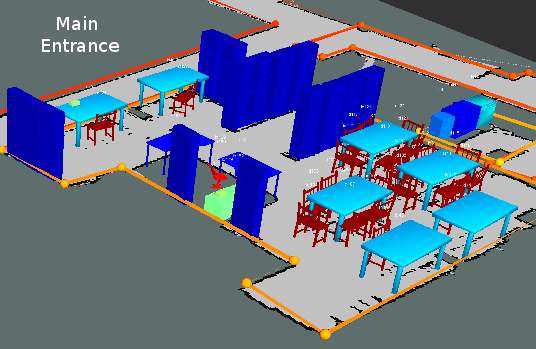
\includegraphics[width=2.5in]{fig/Library01.png}}\\
  \label{fig_library}\caption{The library setting}
\end{figure}

Because of the rules of the library and the nature of the location, the amount of activities is limited.
However, non-considered activities could eventually appear, as giving a greet, using a cellphone, talking, etc.
The amount of objects involved in the environment is also relatively small (books, tables, chairs, laptops, cabinets, etc.).

Our interest is to use this library setting as a test for activity recognition with a mobile robot, and moreover
The problem can be analysed with simple examples via simulation to build the core of a testing system, and later use real data and eventually a mobile robot.
%Libraries tend to share some similarities, there is the possibility to replicate the experiments from this work in other locations.
%This would create landmarks for testing and comparing different approaches, and direct the research towards a more general and better system.

%For the sake of simplicity and as a starting point, lets consider the following abstraction: a linear library (Fig. \ref{}).

%\begin{figure}[h]
%\centering
%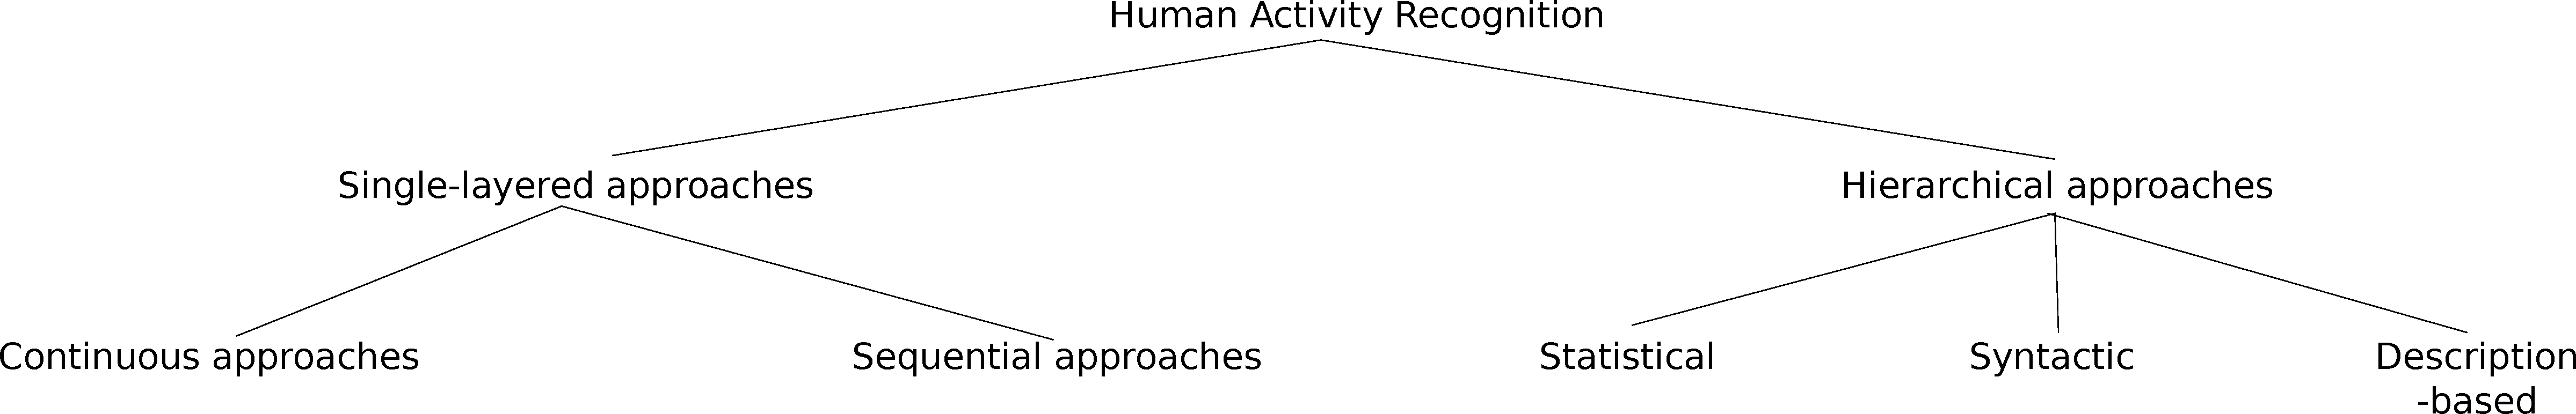
\includegraphics[width=\textwidth]{fig/img_Aggarwal_Taxonomy2.pdf}
%\caption{The taxonomy of research in activity recognition described in \cite{Aggarwal11_HumanActivity}.}
%\label{fig:taxonomy}
%\end{figure}




%Some interesting activities to look at are:

%\begin{description}
%\item[book loan] A person goes to the reception with a book, spend some time on it and later leaves the library with the book.
%\item[book retrieval] A person arrives to the reception with a book and \textit{leaves} the book in the reception.
%\item[study] A person
%\end{description}


%TODO %TODO %TODO

\section{Document organization}

The rest of the document is organized in the following manner.

Chapter \ref{ch_relatedwork} presents related literature to the problem and discusses the results and limitations of previous approaches. The chapter starts with a brief historic presentation of perception in Artificial Intelligence and goes towards the problem of activity recognition. Section\ref{} presents a summary of how the problem of activity recognition has been treated before, and particularly regarding hierarchical description-based approaches, in which ASP is an alternative. In section \ref{sec_DBROB}, some previous works that integrate activity recognition and robotics are reviewed. Finally, in section \ref{sec_DBROB}, ASP is presented as an alternative for solving problems that require knowledge representation and reasoning.

Chapter \ref{ch_research_problem} presents the problem (section \ref{sec_problem}) and the proposed methodology (section \ref{sec_methodology}) to treat it. 

Chapter \ref{ch_eva} presents an experimental approach to evaluate the methodology proposed within this project. By using variations of the library setting environment (section \ref{sec_Library}), the problem can be studied gradually and the main components of an ASP-based approach can be remarked.

Chapter \ref{ch_wp} presents a work plan for the rest of the project duration (2 years) and proposes goals and tasks to achieve them. 

Finally, chapter \ref{ch_conc} presents the conclusions final comments regarding this project and about the developed ideas.









 % Intro & Motivation (Open areas proposed in the literatures)

% Outcome
%\chapter{Related Work}

% 0 - GENERALITIES
% Symbol ground
% Anchoring
% Frame Problem


% 1 - ACTIVITY RECOGNITION
% Historic origins
% Main branches
% Hierarchical pproaches


% 2 - ANSWER SET PROGRAMMING
% General background
% Related work to AR


% 3 - ASP + Robots -> ROSoClingo
% 
 % "Related Work" Literature rev (separated areas, in my case AR + ASP + KRR(incomplete) + Semantic Map)

%================================================
%================================================
%================================================
\chapter{Related Work}

%TODO Intro to the chapter
The general problem to study in this project is activity recognition with a mobile robot. 
In this chapter, relevant related work is reviewed.

In humans, activity recognition is a cognitive skill that can be considered mainly into perception. 
The basis to understand it relies first in Psychology, because it provides the concepts and the evidence of how the mind is constituted (\ref{ch_LitRev_Perception}). 
The next step is to look at the possibilities to mimic a cognitive process into a machine, this problem has been studied widely in Artificial Intelligence. %TODO Add cross reference
In particular, activity recognition has been studied in Computer Vision. %TODO Add cross reference
Finally, the problem has to landed to a robotic stage, making emphasis on the advantages and disadvantages of a robotic platform. %TODO Add cross ref

% 0 - GENERALITIES
% Perception
% Symbol ground
% Anchoring
% Frame Problem

\section{General antecedents - Perception in AI} \label{ch_LitRev_Perception}

Perception, as a cognitive process, has been studied widely in Psychology.
It refers to the process of organizing and interpreting sensory information so that it has a meaning \citep{King2014Psychology}.
Part of the interest is about how sensory information is processed by the brain, and which parts of it are essential.
Also relevant is the domain knowledge that the subject has about a particular context.
Together, the sensory input and the domain knowledge are used to interpret a scene.

%TODO Other interesting examples to discuss later: Plato's Cave, 5 blind men and the elephant, Flatland, Metamorfosis.

Sensory input is important for perception, however, not all the data is equally important to interpret a particular scene and conclusions can still be made, even with partial data.
In \citep{Heider1944_Experimental}, an animated film was created using only moving polygons to demonstrate how the motion of abstract entities could be interpreted by human observers in meaningful ways.
In \citep{Johansson1973_VisualPer}, locomotion patterns of living organisms using visual marks were studied. 
By this mean, the emphasis was put in the qualitative motion description of the marks rather than in the qualitative motion description of the moving body.

In Artificial Intelligence, perception has been treated mostly by the computer vision research community.
Earlier works can be traced back to the 1960s, as part of the effort to mimic human-like intelligence using visual perception components. The main difference between computer vision and image processing has been the desire to recover the three-dimensional structure of the world from images, and to use this as a stepping stone towards full scene understanding \citep{Winston1975_PsyCV}. 


One of the earlier works in 3D reconstruction from a single image is found in \citep{Roberts1963_PhDThesis}.
The developed system was able to reconstruct geometrical bodies with flat surfaces by recognizing the borders of the bodies in the scene and later analysing the shades of their visible surfaces.
%TODO Maybe include Adolfo Guzman Arenas work here. +-
In \citep{Barrow1971_RelatDesc} object recognition was studied by decomposing an image into regions and describing the spatial relations between them, in a more qualitative, rather than the traditional quantitative, approach.

Since the early 1970s, the \textit{block's world} was used as a test scenario for intelligent systems, particularly regarding knowledge representation, reasoning and planning.
In the block's world, an initial state $A$ and a desired state $B$  of the environment are given.
The goal is to autonomously generate a plan to transform $A$ into $B$ by the manipulation of the blocks.
One important characteristic of the problem is that requires a symbolic representation of the scene.
The problem was used as a test case for the robot Shakey \citep{Nilsson84_Shakey}.

%Finally, during the 1980s an approach to perception with emphasis in action feedback became popular
%TODO Complete Active Perception.

%TODO Need to mention QSR.
%TODO Need to mention KRR (ASP, DL, Ontologies, Naive Ph, etc.).


\section{Activity Recognition} 
% Emphasis in the taxomony of the area. I will only describe the taxonomy and give examples. I need to finish with describing the branch that fits better the "robotics" approach, and that will be the next section.

Activity recognition is an important research area in the context of automated perception. 
It has many applications as surveillance, inspection, verification, generation of automated reports, etc.
The application will dictate the approach to follow and the kind on sensors that will be required.

First, regarding sensing, two approaches can be followed, environmental and/or pervasive. 
The first one observes the scene from the distance as it happens with a CCTV camera or a robot. 
The pervasive approach relies on wearable devices to detect the activity of a person from a first person point of view.

Another possible classification of activity recognition systems focuses on how information is processed.
In \citep{Aggarwal11_HumanActivity} a taxonomy is proposed as shown in Fig. \ref{fig:taxonomy}.  

\begin{figure}[h]
\centering
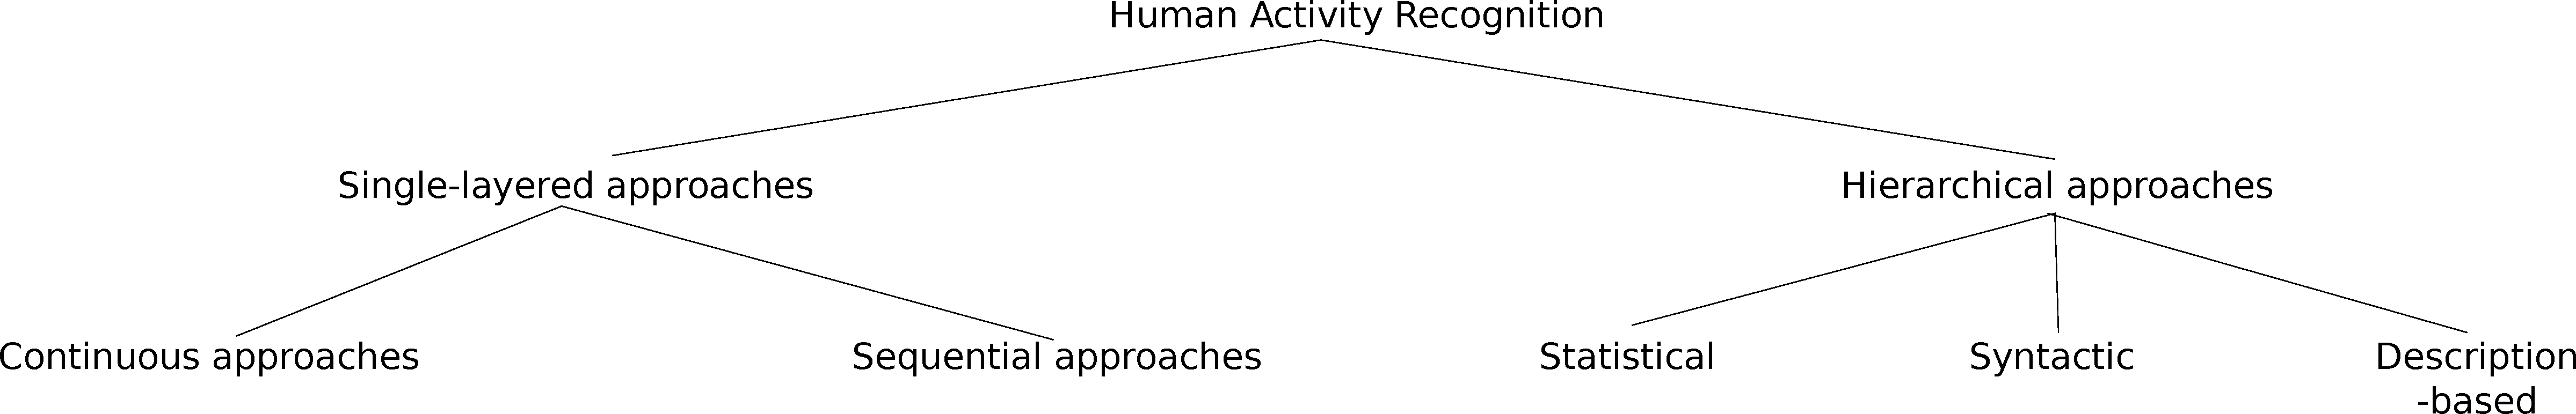
\includegraphics[width=\textwidth]{fig/img_Aggarwal_Taxonomy2.pdf}
\caption{The taxonomy of research in activity recognition described in \cite{Aggarwal11_HumanActivity}.}
\label{fig:taxonomy}
\end{figure}

\subsection{Single-layered approaches}
They represent activities in terms of raw sensory data\footnote{The originaking science psychologyl survey \citep{Aggarwal11_HumanActivity} describes single layered approaches as image-based approaches, but it leaves out the systems with other sensing capabilities (e.g. 3D sensors, sonars, GPS, etc.).
However, they can be included too the activities are represented in terms of raw sensory data patterns.}, because of this, the activity descriptions are trained from datasets.

%Sensory data is processed to obtain particular descriptive features of the scene which are compared with known activity patterns. 
%These patterns can be obtained in a supervised or unsupervised fashion (e.g. common occurrences of a specific action). 
%Most of them are based in computer vision and machine learning techniques.

Single-layered approaches are suitable to recognize short-term and simple activities as gestures, movements of the body or simple interactions with objects. 
This is mainly because the amount of sensory data grows very easily and long-term activities would require to process larger amounts of data. 
Also, because activities are not always performed in the same way, even by the same individual; the shorter the activity, the more accuracy that will be attained.
An finally, because they are dependant on the sensors and on the environmental conditions (e.g. lighting, point of view).


\subsubsection{Continuous approaches\footnote{`Space-time approaches' in \citep{Aggarwal11_HumanActivity}}} % BEFORE: Space-Time approaches

The activities are recognized by analysing continuous sensory data and compare it with an activity pattern.

An activity is represented as a block of data along time where the activity was performed, and it is considered as a whole.
A volume (or hyper-volume) is built by concatenating the sensor readings in time.
The dimension of the data will depend on the sensing capabilities of the system; for example, a video stream would require 3 dimensions $(X,Y,T)$ and a RGBD camera would be able to use 4 dimensions $(X,Y,Z,T)$, etc. %TODO Consider RGB values..., what happens with other dimensions, e.g. temperature?
The sensory input is compared with the activity patterns to measure similarity.
If a threshold is fulfilled, then the activity is labelled.

The advantages of this approach is that it is relatively fast and doesn't require domain knowledge. 
However, it is very dependant of the sensory input, the continuity of the data, how the activity is performed and of the point of view where the scene is being observed. %TODO HOMEWORK: What about interpolating the data in incomplete situations.

There are many examples of this approach.
In \citep{Bobick2001_RecHuMovTemp} a video stream of aerobics exercises was analysed by attaching to every pixel a vector indicating the presence and recency of motion. 
Then the stream was compared online with previously described activities to look for matching. 
In \citep{Ke2007_SpTmpShapeAR}, volumes were built by attaching similar regions of adjacent frames.
Then, the problem was transformed in an object matching problem by comparing the shapes of the volumes (sensory stream and activity patterns).

\subsubsection{Sequential approaches} %TODO Go deeper.

Sequential approaches represent activities as a sequence of states. 
A state is a vector of features observed in the scene in a specific time.
Finally, the sequence is analysed depending on the activity representation.
There are two approaches: exemplar-based and model-based.

In exemplar-based approaches, activities, or a class of them, are represented as a sequence of states. 
Then the sensory input is compared in similarity with the patterns.
An example can be found in \citep{Darrell1993_STGestures}, where states are built from view models.
Templates of activities are from sequences of states associated with a physical change (e.g. rotation and scale).
The dynamics of articulated objects in scene were recognized using the dynamic time warping algorithm (DTW) to the sequence of states.

In model based approaches, the sequence of states is compared with a set of probabilistic models of activities. The models are built assuming a temporal dependence between the states, so the transitions are modelled probabilistically using hidden Markov models (HMM) or dynamic bayesian networks (DBN).

The first work to use HMM to recognize activities was \citep{Yamato1992_RecHA_HMM}. They transformed a video stream into a sequence of vectors of image features. Then every vector was transformed to a symbol using vector quantization. Finally, a set of HMMs were created to model the activities, and their parameters were optimized. 


%TODO %TODO %TODO %TODO %TODO %TODO %TODO %TODO %TODO %TODO %TODO %TODO %TODO %TODO %TODO %TODO 
%TODO %TODO %TODO %TODO %TODO %TODO %TODO %TODO %TODO %TODO %TODO %TODO %TODO %TODO %TODO %TODO 

\subsection{Hierarchical approaches}
Hierarchical approaches for activity recognition refer to those where complex activities are represented in terms of simpler ones. 
Multiple layers are defined to represent activities in different levels of complexity.
Low level activities can be recognized using single-layered approaches. 

Hierarchical approaches are also adequate to represent activities symbolically by using the multi-layered organization to describe semantic relations.
By these means, hierarchical approaches are less dependant to training data and they can integrate domain knowledge more easily.

Hierarchical approaches can be categorized, regarding the applied methodology for recognition as statistical, syntactical and description-based. %TODO Expand.


\subsection{Statistical}
They are based in the hierarchical construction of statistical state-based models, such as HMMs or DBNs.

First the set of activities to work with is defined and organized hierarchically.
Complex activities are defined in terms of simpler ones and so on until everything can be synthesized to atomic actions.
In this way, many layers are created, from atomic actions to complex activities.
In the bottom level, atomic actions are recognized from sensory data using single-layered sequential approaches. 
As a result, a sequence of feature vectors is transformed into a sequence of atomic actions.
This sequence is the input for the next layer, which now will be treated as a new sequence of observations, and the same approach to recognize atomic actions from the first layer will be applied in the second one, and so on.

In \citep{Oliver2002_LayRepHumActRec}, the authors present layered hidden Markov models (LHMMs) for online activity recognition using data from video, sound and keyboard data. 
They divide their system in three layers: the first one is in charge of recognizing features from every source, the second layer trigger short events from the scene, and the last layer is used for longer activities. 
The hierarchical approach showed an improved performance when compared to single-layered systems.
The training data is used more efficiently and it's more easy to add more detail on specific activities.

Some disadvantages of the statistical approaches is their difficulty to model the temporal structure of events (e.g. $A$ occurred `during'/`before'/`after' $B$) and also, because of their sequential nature, is hard to handle multiple concurrent tasks.

\subsubsection{Syntactic}
In the syntactical approach, activities are represented symbolically as a set of production rules generating a string of atomic actions which is later recognized using parsing techniques.
Atomic actions are obtained with a single-layered approach, however, in higher layers, recognition is performed symbolically.
Context-free grammars (CFGs) and stochastic context-free grammars (SCFGs) are some of the techniques that have been used to recognize high level activities.

One limitation of this approach is the difficulty to handle concurrent activities, and also to consider unexpected events that are not integrated in the grammar.

An example can be found in \citep{Ivanov2000_RecVisActSCFG}.
The authors aim to recognize complex activities in sequences of video.
Two layers are defined; in the lower level, atomic actions are recognized using HMMs, and in the upper one uses SCFGs.
The approach showed to be able to handle longer time activity constraints and more robust to uncertain detections in the lower level.


\subsubsection{Description-based}
This approach represent activities as a hierarchy of events, making emphasis in their spatial, temporal and logical structures.

A complex activity is modelled from de occurrence of its sub-events that satisfies certain relations.
The temporal relation between sub-events is usually considered in the representation using Allen's calculus \citep{Allen83_MaintainingKnowledgeTemporal}.
Atomic actions are obtained from




% 2 - ACTIVITY RECOGNITION PROBLEM
% Approaches (camera, wearable device, ubiquitous computing)
% Main branches (single layer, multpiple layer)
% Hierarchical approaches

%\section{Activity Recognition (robots, ASP, QSR, 3D)}
% 1.5 ACTIVITY RECOGNITION WITH A MOBILE ROBOT
%A robot can be roughly conceived as a physical entity capable of sensing and performing actions in the world.
%With this in mind, it seems clear that a robot, with sufficient sensing capabilities, is a good candidate to perform the task.

%\subsection{ASP}

% 2 - ANSWER SET PROGRAMMING
% General background
% Related work to AR


% 3 - ASP + Robots -> ROSoClingo
% 
%================================================
%================================================
%================================================


%\chapter{Research Problem}

\section{Human activity analysis}
% Description of the problem

%TODO Main sentence for the problem

The application domain will dictate the activities to be recognized, the required precision, the sensors to be used and their location (environment located or wearable), the time constraints for deliberation,


% Alternatives for each part
% > Observations
% > Knowledge (where? & how?, I'll do it by hand, but it's important to mention alternatives).
% > Representations
% *** CHECK THE orgnanization from the surveys
%   - Modelling activities in space (QSR)
%   - Modelling activities in time  (QSTR ~ Allen's, Fluent, Event, etc).
%   - Modelling activities semantically (Ontologies + Hierarchies)
% > Inference

% Test example

\section{Proposal} % Or alternatives

% Main parts of the problem

% A - Scene decomposition (locations, objects, persons)
%   > from observations to scene reconstruction

% B - 

% B - Representation 
% Modelling in space (QSR)
% Modelling in time (QSTR)
 % (Mike --> Model & Methodology) % Research Problem (Analysis) (Problem Definition -> Rafee)
%\input{040_Methodology.tex}% * Methodology (Here goes the strategy to face the problem, THE PROPOSAL!!)
%\chapter{Experimental Approach} \label{ch_eva} % Or alternatives

Once presented the problem and a proposed methodology to treat it, some approach is required to test the feasibility of the ideas.
With this in mind, and given the practical interest of the problem, an experimental approach is proposed, using the library example (section \ref{sec_Library}) as a testing case to implement and analyse the proposed ideas. 
The library setting is flexible enough to be stated with different degrees of complexity and putting special emphasis on critical areas (e.g. temporal analysis, incomplete information, etc.).

%In this case, the proposed experimental environment is the library setting described in section \ref{sec_Library} with some simplifications and extensions to emphasize particular parts of the problem.
%By these means, the problem can be divided in smaller

\section{Library Example}

The library setting, presented in section \ref{sec_Library}, provides a good testing environment.
It has some desired qualities for experimentation, principally, a bounded space and a compact set of activities.
%Now, some incremental

Let first introduce a simplified version of the library setting.
%If we reuse the library example from chapter 1 it is worth to show how the presented approach applies to that problem.
%With this in mind, let's first make a simplification of the example.
In Figure \ref{fig:ex_library} is presented a \textit{linear} library. 
It has five connected and consecutive regions: (A) main entrance, (B) printing area, (C) reception, (D) bookshelf and (E) common area.

\begin{figure}[h]
\centering
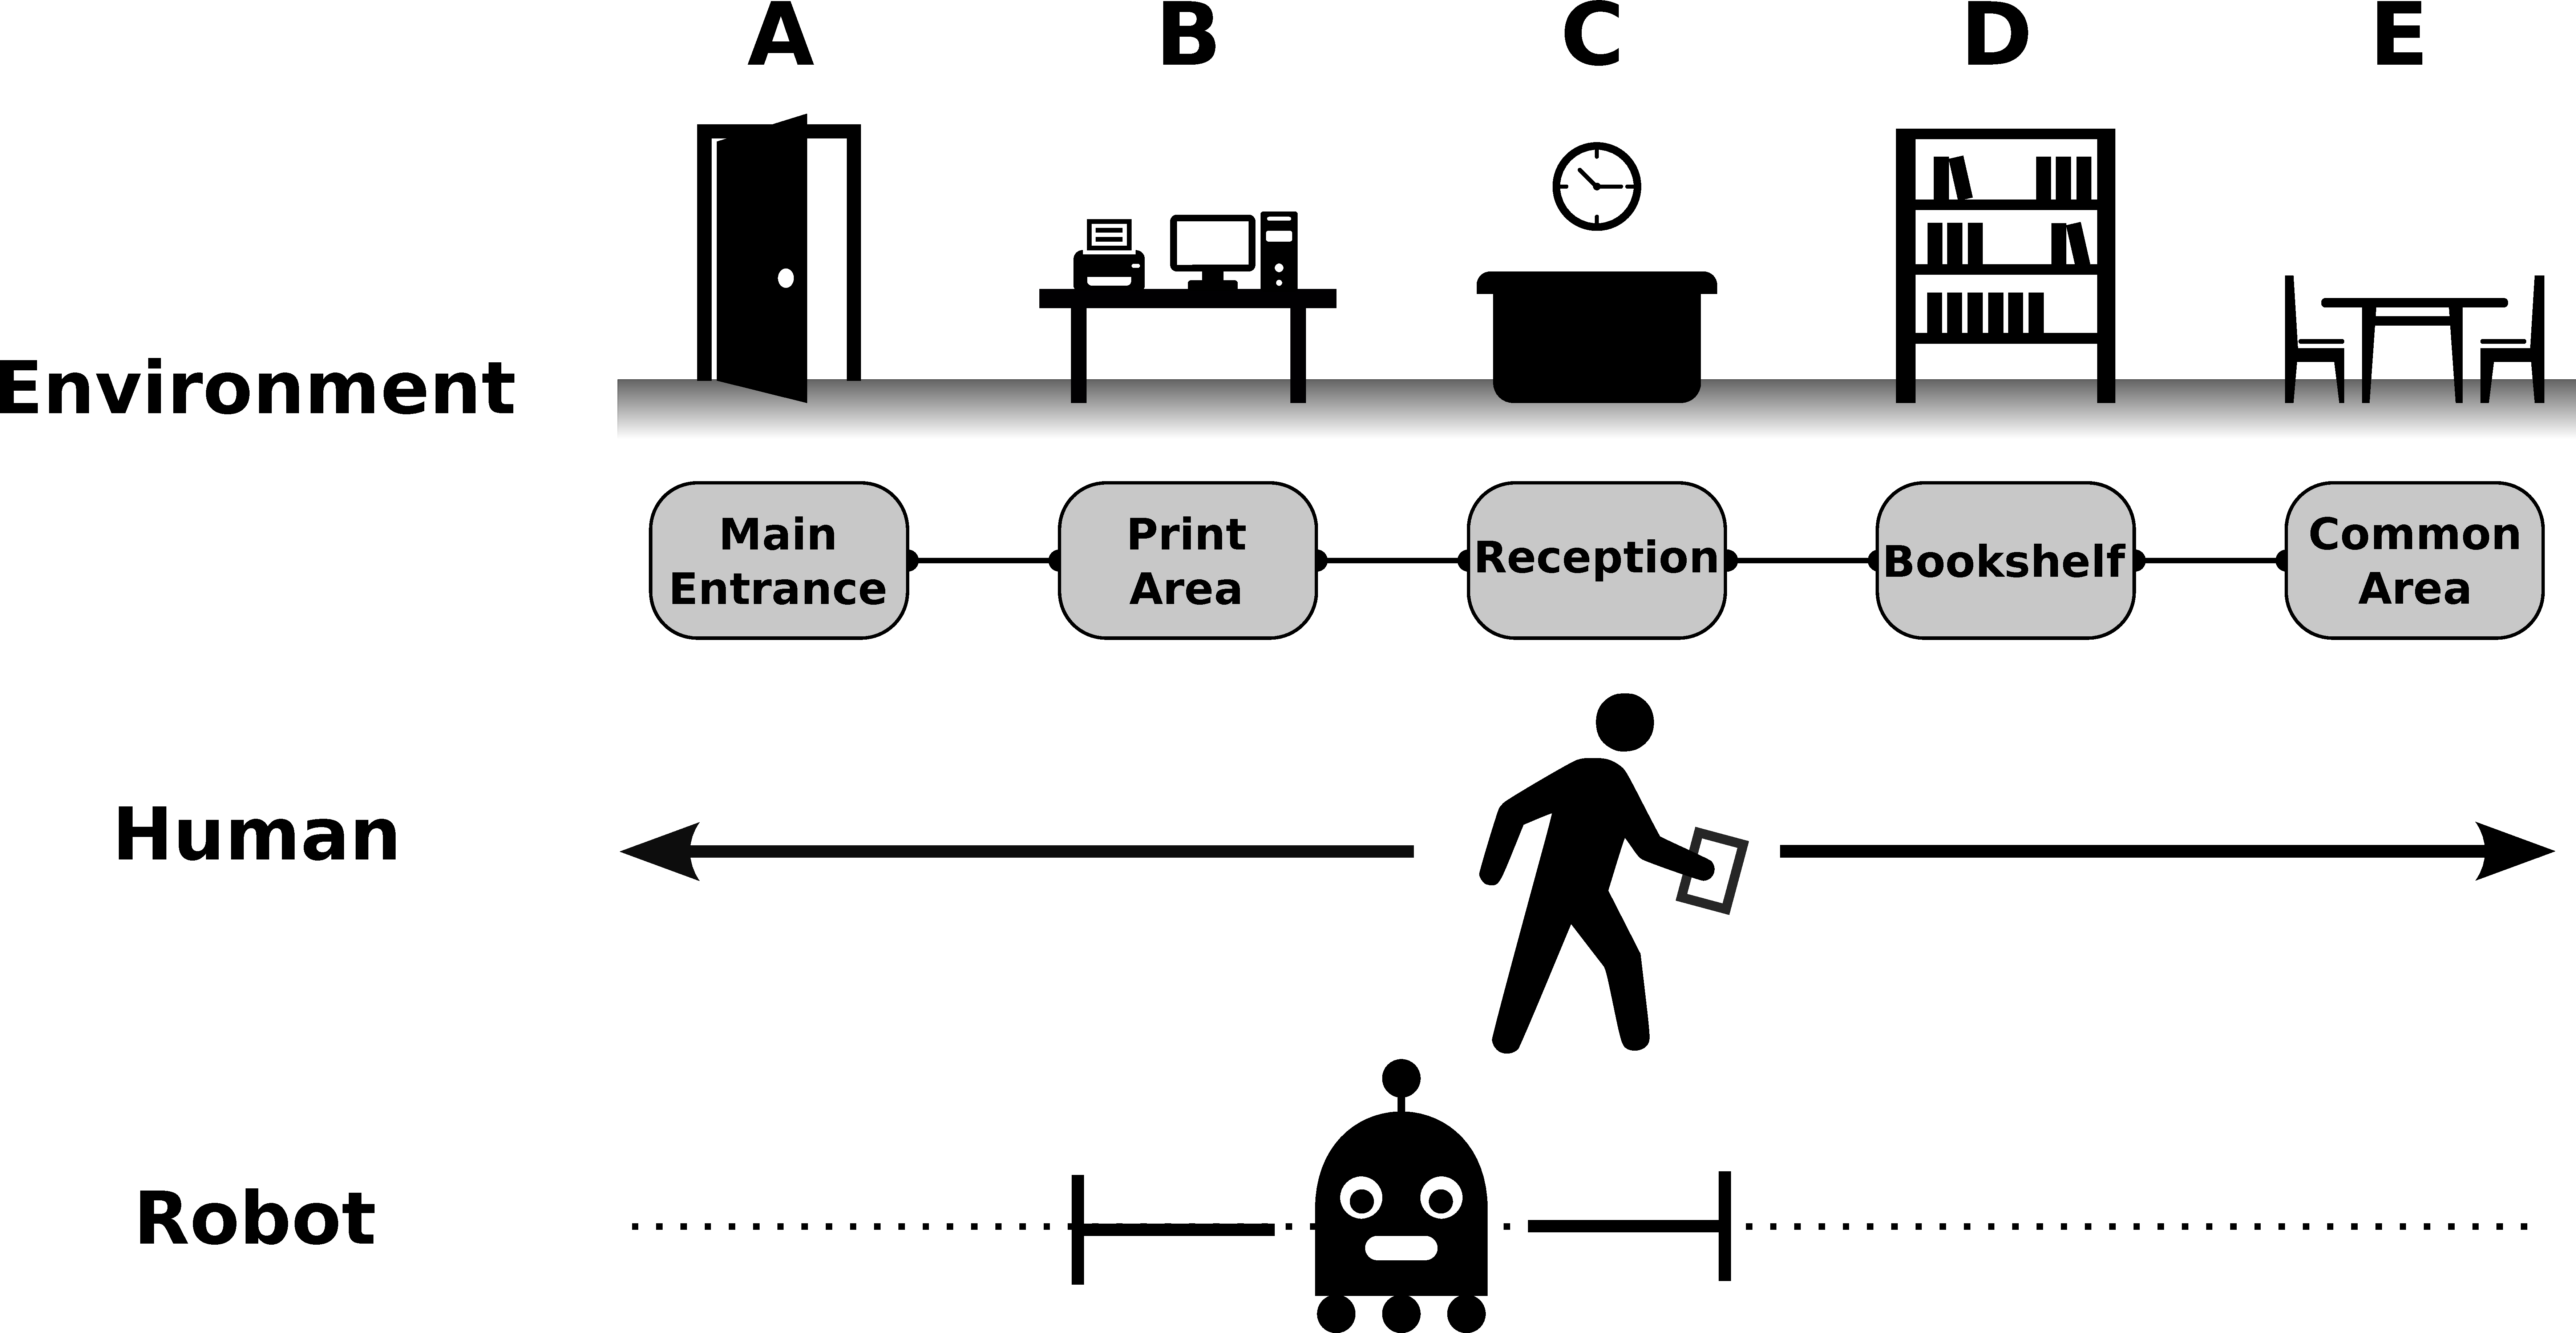
\includegraphics[width=\textwidth]{fig/ex_library.pdf}
\caption{Simplified library setting}
\label{fig:ex_library}
\end{figure}


In this simplified world a person and a robot can move linearly to any region, and they don't obstruct each other.
An activity is performed by a person by visiting regions in a proper order and spending \textit{enough} time on each of them, these intervals are considered within the activity representation.
The challenge here is to recognize the activities of the person.
The robot have an active role by tracking and following the human through the regions he visits and labelling this within its internal world model.

The following activities can be defined:

\begin{description}
\item[print]$B$ 
\item[study]$D \rightarrow E \rightarrow D$
\item[bookLoan]$D \rightarrow C$
\item[bookRetrieval]$C$
\item[requestAssistance]$C$
\end{description}

Now the problem is, given a particular state of the world, to recognize the ongoing activity.
The representations can complete by considering all the occurring states for an activity, but in reality, a robot can realize about the activity in when an intermediate state is occurring. For example, the robot may be watching someone standing in front of the Bookshelf (region $D$), at this point there are two possible activities to consider: \textit{bookLoan} or \textit{study}, because $D$ is an ambiguous state. In this case, the future state will decide the activity.

Now, some extensions can be induced to this simplified world.
\begin{itemize}
\item A robot can have limited sensors, so it will only be able to sense two regions at the same time. 
So, some activeness is required. For example, being observed a person going towards the common area, the robot can move to confirm the position of the person.
\item Handling multiple subjects in the scene, complicates the problem. The robot won't be able to observe all of them, but may try to maximize the observations and after labelling some individuals may go back and sense the rest of the subjects.
\item Object recognition can be induced to disambiguate activities. For example, two activities with the same region description can have an additional parameter regarding the presence of an object. In these cases, a robot can go an confirm the presence or absence of the object to discriminate its hypotheses. 
\end{itemize} 

\subsection{Experimental stages}

Four different stages of the library setting are presented that enables progressive analysis and testing of the ideas within this project. These stages goes from simplistic simulations towards a real robotic platform performing activity recognition, which is the ultimate goal of the research in this project.


\subsubsection{Terminal Simulation}
An implementation of the library setting in as a \textit{terminal} simulation.
The activity representations are defined explicitly and the world states can be defined explicitly as well, or generated with another program.
\begin{itemize}
\item[Pros:]
\item Simplicity
\item Flexible to rapidly implement different cases
\item Simple agents (humans and robot) can be modelled.
\item Controllable parameters
\item Repeatability
\end{itemize}
\begin{itemize}
\item[Cons:]
\item Non realistic data
\end{itemize}

\subsubsection{MORSE Simulation}
MORSE is a simulation environment designed explicitly for robotics which allows compatibility of between the simulation environment and real robotic platforms. An implementation a 3D robotic simulator would enable to test more realistic cases which also can be repeated to test different approaches. Robots, human avatars and sensors are available to be controlled and to retrieve data. 

\begin{itemize}
\item[Pros:]
\item Robotic oriented environment
\item More realistic representations of activities
\item Controllable parameters
\item Repeatability
\item Straight forward software integration
\end{itemize}
\begin{itemize}
\item[Cons:]
\item Non realistic data
\item Integration takes time
\end{itemize}


\subsubsection{Dataset Analysis}
Datasets for activity recognition are available (see \citep{Tenorth2009_TUMKData,Liu2011_BenchmarkDatasHAR}). They provide a standardized test bed for different techniques. While it would difficult to find datasets that take in consideration a robotic platform, it is worth to test individual parts of the overall system to compare with other approaches.
\begin{itemize}
\item[Pros:]
\item Standard data test bed and benchmarking
\item Results available for comparison
\item Repeatability
\end{itemize}
\begin{itemize}
\item[Cons:]
\item Analysis \textit{a posteriori}
\item No robot present, so no active behaviour would be possible
\item Data relies on specific conditions
\end{itemize}

\subsubsection{Robot}
The end goal of this project is to provide robots with the capacity to recognize human activities and understand the relation between them and the environment. This goal far beyond the scope of this project. However, experimentation with real robotic systems is an important step in that direction as real environment conditions are difficult to replicate, and also because the application of these king of systems is oriented mostly in this direction.
\begin{itemize}
\item[Pros:]
\item Real conditions
\item New problems can emerge from non considered situations
\end{itemize}
\begin{itemize}
\item[Cons:]
\item Difficult repeatability
\item Dynamic and non deterministic environment
\item Difficult implementation and slow experimentation
\item Noisy and Uncertain data
\end{itemize}


%TODO %TODO %TODO Complete the example.











% Main parts of the problem

% A - Scene decomposition (locations, objects, persons)
%   > from observations to scene reconstruction

% B - 

% B - Representation 
% Modelling in space (QSR)
% Modelling in time (QSTR)











% Evaluation (Pros + Cons, Possible failures, etc.)
%\chapter{Work Plan}

The main goal of this project is to present a concise study of the integration of ASP and robotics to treat the problem of activity recognition.
By this mean, a work plan should be submitted as a guide line to direct future activities and to measure the progress in the the project. In the following sections, two plans are are presented, short-term (6 months) and long-term (2 years). The proposed goals are distributed in three groups:

First \textit{project goals} are those which moves forward the research project. 
As the direction of research is now clear (ASP-based activity recognition with a mobile robot), and the literature review is considerably up to date, these goals are in the sense of the implementation, testing and analysis of the proposed methodology, to find the paths that conduce to better results. 
At the beginning these tasks will be simple and look to proof the feasibility of the proposed ideas. 
In the final stages, the tasks will be driving the project towards more realistic cases and/or towards specific problems that proof to be relevant.

\textit{Research goals} are those which serve for research training purposes and those enable the participation of the current project in activities within the research community, e.g. conferences, research school meetings, presentations, academic writing, etc.

Finally, the \textit{academic responsibilities} are conformed with those tasks that are mandatory for PhD students within an academic program.


\section{Long-term Plan}

%In the long-term, the main goal is the proper completion of the project by the fulfilment of minor goals. 

\subsection{Project Goals}

\subsubsection*{T1 - Library Setting 01: Terminal simulation}
\paragraph{Objectives}
\begin{itemize}
\item Start the implementation of an activity recognition system using the 2D library setting.
\item Explore simple representations of activities.
\item Get familiar with ASP tools (Clingo, ROSoClingo).
\end{itemize}
\paragraph{Tasks}
\begin{enumerate}
\item The implementation of a simple (terminal) activity recognition system using ASP tools (Potassco).
\item Test different representations of activities based on the interaction between spaces (regions) and humans (positions).
\item Test sequential representation of activities, i.e. a human visiting different locations.
\item Consider objects in scene and within the activity representations.
%\item \textit{Optional} Add visualisation software, e.g. NetLogo.
%\item \textit{Optional} Consider simple robot activity.
\end{enumerate}


\subsubsection*{T2 - Library Setting 02: MORSE Simulation}
\paragraph{Objectives}
\begin{itemize}
\item Implement a more realistic 3D simulation of the library setting.
\item Integrate ROS, Potassco and MORSE in a system.
\item Extend the representation of activities to a 3D environment; i.e. start considering geometrical entities as regions, trajectories, etc.
\end{itemize}
\paragraph{Tasks}
\begin{enumerate}
\item Create the library setting in MORSE and attack one robot to the environment.
\item Integrate ROS and Potassco (via ROSoClingo) with the MORSE simulation.
\item Explore spatial
\end{enumerate}


\subsection{Research Goals}

\subsection{Academic Goals}







\section{Short-term plan - 6 months}

In the short term, the goals will be focused in an introductory p, implementation and experimentation of the proposed methodology.
Proper mastery of ASP is desired to make a proper use of its capabilities.

The work will be oriented with two purposes.

\begin{itemize}
\item Get a deeper understanding of ASP, and particularly in the context of robotics.
\item Board the problem of activity recognition with simple cases.
\end{itemize}



The first point is mentioned because ASP has a central role in this project, is important to complete a proper analysis from insight about the possibilities and requirements to achieve the goal.
This includes the possible synergy with ASP and other techniques (e.g. probabilistic approaches) to improve the possibilities of an overall system.

Regarding the second point, activity recognition is the problem to treated.
A simple solution should be built, in order to have a platform for testing and also build more complex implementations.

\subsection{Short-term table}

\begin{landscape}

\begin{ganttchart}[hgrid,
%vgrid={*1{blue, ultra thick}, dotted},
vgrid,
x unit=7mm,time slot format=isodate, compress calendar]{2015-04-02}{2017-06-31}
\gantttitlecalendar{year, month} \\
%\gantttitlecalendar{year, month } \\
%\ganttgroup{Absences}{2015-04-02}{2015-04-06} \\
\ganttbar{}{2015-04-06}{2015-01-31}
\end{ganttchart}



%\ganttset{%
%calendar week text={W~\currentweek}
%}
%\begin{ganttchart}[hgrid,vgrid,x unit=4mm,time slot format=isodate]{2015-04-02}{2015-10-02}
%\gantttitlecalendar{year, month=shortname, week} \\
%%\gantttitlecalendar{year, month } \\
%\ganttbar{}{2015-04-06}{2015-07-02}
%\end{ganttchart}



%\begin{ganttchart}{1}{12}
%\gantttitle{2015}{12} \\
%\gantttitlelist{1,...,12}{1} \\
%\ganttgroup{Group 1}{1}{7} \\
%\ganttbar{Task 1}{1}{2} \\
%%\ganttlinkedbar{Task 2}{3}{7} \ganttnewline
%%\ganttmilestone{Milestone}{7} \ganttnewline
%%\ganttbar{Final Task}{8}{12}
%%\ganttlink{elem2}{elem3}
%%\ganttlink{elem3}{elem4}
%\end{ganttchart}




%\begin{ganttchart}{1}{12}
%\gantttitle{2015}{12} \\
%\gantttitlelist{1,...,12}{1} \\
%\ganttgroup{Group 1}{1}{7} \\
%\ganttbar{Task 1}{1}{2} \\
%\ganttlinkedbar{Task 2}{3}{7} \ganttnewline
%\ganttmilestone{Milestone}{7} \ganttnewline
%\ganttbar{Final Task}{8}{12}
%\ganttlink{elem2}{elem3}
%\ganttlink{elem3}{elem4}
%\end{ganttchart}




%\newpage

\end{landscape}




\begin{verbatim}
1 - Mini-World Simulation

2 - Library 3D Simulation

3 - Library Datasets (actors & controlled environment)

4 - Library (real environment)
\end{verbatim}


%\begin{itemize}
%\item Experiments 1 - Proof of concept
% \begin{itemize}
% \item Simulation - Simple ASP console example
% \item Simulation - Morse
% \end{itemize}
%\item Experiments 2 - Improve first experimental phase
% \begin{itemize}
% \item Expand activity representation and repertoire to handle more complicated cases
% \item Implement approach
% \end{itemize}
%\end{itemize}






% * Work Plan (Research Goals+- --> Paul Engelfield)
% Work Done (so far)
% Timetable

% MAke a Timeline of AR
% Check "Paul Engelfield" --> Good Report

% *5min sketch of the report at the begining

% Bibliography
\clearpage
\bibliographystyle{abbrvnat}
\bibliography{/home/kilgore/Dropbox/Public/Docs/mabp_bibliography.bib}
%\bibliography{Bibliography.bib}


\end{document}
